% -*- coding: utf-8 -*-
Este apéndice recoge soluciones de una selección de ejercicios de los temas~\ref{cap:dn-prop}, \ref{cap:sem-prop}, \ref{cap:dn-lpo}, \ref{cap:sem-lpo} y~\ref{cap:tableaux}. Las derivaciones no son únicas: si tu solución es distinta, comprueba con el asistente web que cada línea está bien justificada. Los ejercicios del tema~\ref{cap:meta-prop} ya incluyen soluciones guiadas en el propio tema.

\section{Tema 1: deducción natural en lógica proposicional}

\begin{solucion}{e1-10}
\begin{center}
$\begin{nd}[rules=myrules]
    \hypo [1] {1} {(p \land q) \to r} \by{Prem.}{}
    \open
        \hypo [2] {2} {p} \by{Hip.}{}
        \open
            \hypo [3] {3} {q} \by{Hip.}{}
            \have [4] {4} {p \land q} \ai{2, 3}
            \have [5] {5} {r} \ce{1, 4}
        \close
        \have [6] {6} {q \to r} \ci{3-5}
    \close
    \have [7] {7} {p \to (q \to r)} \ci{2-6}
\end{nd}$
\end{center}
\end{solucion}

\begin{solucion}{e1-15}
\begin{center}
$\begin{nd}[rules=myrules]
    \hypo [1] {1} {p \lor q} \by{Prem.}{}
    \hypo [2] {2} {\lnot p} \by{Prem.}{}
    \open
        \hypo [3] {3} {p} \by{Hip.}{}
        \have [4] {4} {\bot} \ne{2, 3}
        \have [5] {5} {q} \x{4}
    \close
    \open
        \hypo [6] {6} {q} \by{Hip.}{}
        \have [7] {7} {q} \r{6}
    \close
    \have [8] {8} {q} \oe{1, 3-5, 6-7}
\end{nd}$
\end{center}
\end{solucion}

\begin{solucion}{e1-16}
Primero derivamos $\neg p$ (si $p$, la premisa da $\neg p$) y después, con la premisa, $p$:
\begin{center}
$\begin{nd}[rules=myrules]
    \hypo [1] {1} {p \leftrightarrow \lnot p} \by{Prem.}{}
    \open
        \hypo [2] {2} {p} \by{Hip.}{}
        \have [3] {3} {\lnot p} \be{1, 2}
        \have [4] {4} {\bot} \ne{3, 2}
    \close
    \have [5] {5} {\lnot p} \ni{2-4}
    \have [6] {6} {p} \be{1, 5}
    \have [7] {7} {\bot} \ne{5, 6}
\end{nd}$
\end{center}
\textbf{Comentario.} Si $p$ es «esta oración es falsa», la premisa dice que la oración es verdadera si y solo si es falsa. La derivación muestra que esa premisa es contradictoria: es la estructura lógica de la paradoja del mentiroso.
\end{solucion}

\begin{solucion}{e1-18}
\begin{center}
$\begin{nd}[rules=myrules]
    \hypo [1] {1} {\lnot(p \lor q)} \by{Prem.}{}
    \open
        \hypo [2] {2} {p} \by{Hip.}{}
        \have [3] {3} {p \lor q} \oi{2}
        \have [4] {4} {\bot} \ne{1, 3}
    \close
    \have [5] {5} {\lnot p} \ni{2-4}
    \open
        \hypo [6] {6} {q} \by{Hip.}{}
        \have [7] {7} {p \lor q} \oi{6}
        \have [8] {8} {\bot} \ne{1, 7}
    \close
    \have [9] {9} {\lnot q} \ni{6-8}
    \have [10] {10} {\lnot p \land \lnot q} \ai{5, 9}
\end{nd}$
\end{center}
\end{solucion}

\begin{solucion}{e1-22}
Sin usar LEM, suponemos la negación de la conclusión y aplicamos IP:
\begin{center}
$\begin{nd}[rules=myrules]
    \open
        \hypo [1] {1} {\lnot(p \lor \lnot p)} \by{Hip. IP}{}
        \open
            \hypo [2] {2} {p} \by{Hip.}{}
            \have [3] {3} {p \lor \lnot p} \oi{2}
            \have [4] {4} {\bot} \ne{1, 3}
        \close
        \have [5] {5} {\lnot p} \ni{2-4}
        \have [6] {6} {p \lor \lnot p} \oi{5}
        \have [7] {7} {\bot} \ne{1, 6}
    \close
    \have [8] {8} {p \lor \lnot p} \ip{1-7}
\end{nd}$
\end{center}
\end{solucion}

\begin{solucion}{e1-24}
\begin{center}
$\begin{nd}[rules=myrules]
    \hypo [1] {1} {(p \to q) \to p} \by{Prem.}{}
    \open
        \hypo [2] {2} {\lnot p} \by{Hip. IP}{}
        \open
            \hypo [3] {3} {p} \by{Hip.}{}
            \have [4] {4} {\bot} \ne{2, 3}
            \have [5] {5} {q} \x{4}
        \close
        \have [6] {6} {p \to q} \ci{3-5}
        \have [7] {7} {p} \ce{1, 6}
        \have [8] {8} {\bot} \ne{2, 7}
    \close
    \have [9] {9} {p} \ip{2-8}
\end{nd}$
\end{center}
\textbf{Comentario.} La ley de Peirce no puede demostrarse sin una regla clásica como IP (no es válida en lógica intuicionista).
\end{solucion}

\begin{solucion}{e1-29}
Una derivación sistemática se obtiene con el método de Kalmár: véase el ejemplo~\ref{ej:kalmar-linealidad} del tema~\ref{cap:meta-prop}. Una más breve usa LEM sobre $q$: si $q$, se obtiene $p \to q$ (suponiendo $p$ y reiterando $q$); si $\neg q$, se obtiene $q \to p$ (suponiendo $q$, $\bot$ con $\neg q$ y X); en ambos casos se obtiene la disyunción por $\lor$I, y LEM permite concluirla fuera de las cajas.
\end{solucion}

\section{Tema 2: semántica de la lógica proposicional}

\begin{solucion}{e2-negcond}
$p \land q \equiv \neg(p \to \neg q)$:
\begin{center}
\begin{tabular}{cc|c|c|c|c}
$p$ & $q$ & $\neg q$ & $p \to \neg q$ & $\neg(p \to \neg q)$ & $p \land q$ \\
\hline
1 & 1 & 0 & 0 & 1 & 1 \\
1 & 0 & 1 & 1 & 0 & 0 \\
0 & 1 & 0 & 1 & 0 & 0 \\
0 & 0 & 1 & 1 & 0 & 0
\end{tabular}
\end{center}
\end{solucion}

\begin{solucion}{e2-negdisy}
$p \leftrightarrow q \equiv \neg(\neg p \lor \neg q) \lor \neg(p \lor q)$. En efecto, por De Morgan $\neg(\neg p \lor \neg q) \equiv p \land q$ y $\neg(p \lor q) \equiv \neg p \land \neg q$, y $p \leftrightarrow q$ es verdadera exactamente cuando $p$ y $q$ son ambas verdaderas o ambas falsas.
\end{solucion}

\begin{solucion}{e2-consec}
\begin{enumerate}[(a)]
    \item No es válida. Contraejemplo: $v(p) = 0$, $v(q) = 1$ (las premisas son verdaderas y $\neg q$ es falsa).
    \item No es válida. Contraejemplo: $v(p) = 1$, $v(q) = 1$, $v(r) = 0$.
    \item Es válida (si $v(\neg p) = 1$, la única forma de que $p \lor q$ sea verdadera es $v(q) = 1$). La derivación es la del ejercicio~\ref{e1-15}.
    \item Es válida. Para un contraejemplo necesitaríamos $v(q) = 1$, $v(p) = 1$ y $v(r) = 0$, pero entonces $v(q \to r) = 0$ y $v(p \to (q \to r)) = 0$. Derivación:
    \begin{center}
    $\begin{nd}[rules=myrules]
        \hypo [1] {1} {p \to (q \to r)} \by{Prem.}{}
        \hypo [2] {2} {p \land \lnot r} \by{Prem.}{}
        \have [3] {3} {p} \ae{2}
        \have [4] {4} {\lnot r} \ae{2}
        \have [5] {5} {q \to r} \ce{1, 3}
        \open
            \hypo [6] {6} {q} \by{Hip.}{}
            \have [7] {7} {r} \ce{5, 6}
            \have [8] {8} {\bot} \ne{4, 7}
        \close
        \have [9] {9} {\lnot q} \ni{6-8}
    \end{nd}$
    \end{center}
    \item Es válida. Para un contraejemplo necesitaríamos $v(p \lor r) = 1$ y $v(q) = 0$. Pero entonces $v(p) = 1$ o $v(r) = 1$, y en ambos casos una de las premisas, $p \to q$ o $r \to q$, sería falsa. Derivación:
    \begin{center}
    $\begin{nd}[rules=myrules]
        \hypo [1] {1} {p \to q} \by{Prem.}{}
        \hypo [2] {2} {r \to q} \by{Prem.}{}
        \open
            \hypo [3] {3} {p \lor r} \by{Hip.}{}
            \open
                \hypo [4] {4} {p} \by{Hip.}{}
                \have [5] {5} {q} \ce{1, 4}
            \close
            \open
                \hypo [6] {6} {r} \by{Hip.}{}
                \have [7] {7} {q} \ce{2, 6}
            \close
            \have [8] {8} {q} \oe{3, 4-5, 6-7}
        \close
        \have [9] {9} {(p \lor r) \to q} \ci{3-8}
    \end{nd}$
    \end{center}
\end{enumerate}
\end{solucion}

\begin{solucion}{e2-formal}
\begin{enumerate}[(a)]
    \item $f$: «iré a la fiesta»; $i$: «me invitan». $f \to i$.
    \item $e$: «apruebo el examen»; $a$: «apruebo la asignatura». $a \to e$. Esta fórmula dice que aprobar el examen es condición necesaria para aprobar la asignatura, y no dice que sea suficiente. La segunda parte del enunciado no puede añadirse como $\neg(e \to a)$, porque esa fórmula equivale a $e \land \neg a$, que afirma algo que el enunciado no dice: que apruebo el examen y suspendo la asignatura. Que una condición $C$ no sea suficiente para $P$ es una afirmación general (puede cumplirse $C$ sin que se cumpla $P$) que la lógica proposicional no recoge; en lógica de primer orden se expresaría con cuantificadores.
    \item $s$: «saldremos de excursión»; $l$: «llueve». $\neg l \to s$ (o $s \lor l$).
    \item $k$: «Kant acepta el argumento ontológico»; $h$: «Hume acepta el argumento ontológico». $\neg k \land \neg h$.
    \item $n$: «el conocimiento es innato»; $a$: «el conocimiento es adquirido por la experiencia». $\neg(n \land a)$. (El «no puede» modal se pierde en la formalización).
    \item $e$: «Hume es empirista»; $r$: «Hume rechaza las ideas innatas». $e \leftrightarrow r$.
\end{enumerate}
\end{solucion}

\begin{solucion}{e2-arg}
Apartados (a)--(c):
\begin{enumerate}[(a)]
    \item $c$: «voy al cine»; $l$: «acabo pronto de limpiar la casa»; $a$: «me acompañas». Premisas $c \to l$ y $a \to c$; conclusión $a \to l$. Es válido (silogismo hipotético): para un contraejemplo necesitaríamos $v(a) = 1$ y $v(l) = 0$; entonces la segunda premisa exige $v(c) = 1$, y la primera sería falsa. Derivación:
    \begin{center}
    $\begin{nd}[rules=myrules]
        \hypo [1] {1} {c \to l} \by{Prem.}{}
        \hypo [2] {2} {a \to c} \by{Prem.}{}
        \open
            \hypo [3] {3} {a} \by{Hip.}{}
            \have [4] {4} {c} \ce{2, 3}
            \have [5] {5} {l} \ce{1, 4}
        \close
        \have [6] {6} {a \to l} \ci{3-5}
    \end{nd}$
    \end{center}
    \item $b$: «hace buen tiempo»; $p$: «iremos a la playa». Premisas $b \to p$ y $p$; conclusión $b$. No es válido (afirmación del consecuente): la fila $v(b) = 0$, $v(p) = 1$ es un contraejemplo.
    \item $m$: «el mundo es redondo»; $b$: «tengo un barco»; $n$: «navego alrededor del mundo». Premisas $(m \land b) \to n$ y $b \land \neg n$; conclusión $\neg m$. Es válido: para un contraejemplo necesitaríamos $v(m) = 1$; la segunda premisa exige $v(b) = 1$ y $v(n) = 0$, y entonces la primera sería falsa. Derivación:
    \begin{center}
    $\begin{nd}[rules=myrules]
        \hypo [1] {1} {(m \land b) \to n} \by{Prem.}{}
        \hypo [2] {2} {b \land \lnot n} \by{Prem.}{}
        \have [3] {3} {b} \ae{2}
        \have [4] {4} {\lnot n} \ae{2}
        \open
            \hypo [5] {5} {m} \by{Hip.}{}
            \have [6] {6} {m \land b} \ai{5, 3}
            \have [7] {7} {n} \ce{1, 6}
            \have [8] {8} {\bot} \ne{4, 7}
        \close
        \have [9] {9} {\lnot m} \ni{5-8}
    \end{nd}$
    \end{center}
\end{enumerate}
\end{solucion}

\begin{solucion}{e2-vf2}
Es falsa. Si $\Gamma$ es insatisfacible, no hay ninguna interpretación que haga verdaderas a la vez todas sus fórmulas, de modo que $\Gamma \models A$ y $\Gamma \models \neg A$ se cumplen ambas (por vacuidad). Por ejemplo, con $\Gamma = \{p, \neg p\}$ tenemos $\Gamma \models q$ y $\Gamma \models \neg q$. La afirmación sí es verdadera si $\Gamma$ es satisfacible.
\end{solucion}

\begin{solucion}{e2-cuest}
\begin{enumerate}[(a)]
    \item $\{A\} \models B$ es verdadera: $B$ es verdadera en toda interpretación (y, además, ninguna interpretación hace verdadera a $A$). $\{B\} \models A$ es falsa: cualquier interpretación hace verdadera a $B$ y falsa a $A$.
    \item $\{A, B\} \models C$ se cumple: si una interpretación hiciera verdaderas $A$ y $B$ y falsa $C$, satisfaría $\{A, B, \neg C\}$. Por la misma razón se cumple $\{A, \neg C\} \models \neg B$. En cambio, $\{A, B\} \models \neg C$ no se cumple necesariamente: con $A = p$, $B = q$ y $C = p$, el conjunto $\{p, q, \neg p\}$ es insatisfacible, pero la interpretación $v(p) = v(q) = 1$ hace verdaderas $p$ y $q$ y falsa $\neg p$.
\end{enumerate}
\end{solucion}

\section{Tema 4: deducción natural en lógica de primer orden}

\begin{solucion}{e4-1}
\begin{center}
$\begin{nd}[rules=myrules]
    \hypo [1] {1} {\forall x (M(x) \to \lnot P(x))} \by{Prem.}{}
    \hypo [2] {2} {\forall x (S(x) \to M(x))} \by{Prem.}{}
    \open
        \hypo [3] {3} {S(c)} \by{Hip.}{}
        \have [4] {4} {S(c) \to M(c)} \Ae{2}
        \have [5] {5} {M(c)} \ce{4, 3}
        \have [6] {6} {M(c) \to \lnot P(c)} \Ae{1}
        \have [7] {7} {\lnot P(c)} \ce{6, 5}
    \close
    \have [8] {8} {S(c) \to \lnot P(c)} \ci{3-7}
    \have [9] {9} {\forall x (S(x) \to \lnot P(x))} \Ai{8}
\end{nd}$
\end{center}
\end{solucion}

\begin{solucion}{e4-8}
\begin{center}
$\begin{nd}[rules=myrules]
    \hypo [1] {1} {\exists x (P(x) \lor Q(x))} \by{Prem.}{}
    \open
        \hypo [2] {2} {P(c) \lor Q(c)} \by{Hip. testigo $c$}{}
        \open
            \hypo [3] {3} {P(c)} \by{Hip.}{}
            \have [4] {4} {\exists x P(x)} \Ei{3}
            \have [5] {5} {\exists x P(x) \lor \exists x Q(x)} \oi{4}
        \close
        \open
            \hypo [6] {6} {Q(c)} \by{Hip.}{}
            \have [7] {7} {\exists x Q(x)} \Ei{6}
            \have [8] {8} {\exists x P(x) \lor \exists x Q(x)} \oi{7}
        \close
        \have [9] {9} {\exists x P(x) \lor \exists x Q(x)} \oe{2, 3-5, 6-8}
    \close
    \have [10] {10} {\exists x P(x) \lor \exists x Q(x)} \Ee{1, 2-9}
\end{nd}$
\end{center}
\end{solucion}

\begin{solucion}{e4-12}
\begin{center}
$\begin{nd}[rules=myrules]
    \hypo [1] {1} {\forall x \forall y (R(x, y) \to R(y, x))} \by{Prem.}{}
    \hypo [2] {2} {\forall x \forall y \forall z ((R(x, y) \land R(y, z)) \to R(x, z))} \by{Prem.}{}
    \hypo [3] {3} {\forall x \exists y R(x, y)} \by{Prem.}{}
    \have [4] {4} {\exists y R(a, y)} \Ae{3}
    \open
        \hypo [5] {5} {R(a, b)} \by{Hip. testigo $b$}{}
        \have [6] {6} {\forall y (R(a, y) \to R(y, a))} \Ae{1}
        \have [7] {7} {R(a, b) \to R(b, a)} \Ae{6}
        \have [8] {8} {R(b, a)} \ce{7, 5}
        \have [9] {9} {\forall y \forall z ((R(a, y) \land R(y, z)) \to R(a, z))} \Ae{2}
        \have [10] {10} {\forall z ((R(a, b) \land R(b, z)) \to R(a, z))} \Ae{9}
        \have [11] {11} {(R(a, b) \land R(b, a)) \to R(a, a)} \Ae{10}
        \have [12] {12} {R(a, b) \land R(b, a)} \ai{5, 8}
        \have [13] {13} {R(a, a)} \ce{11, 12}
    \close
    \have [14] {14} {R(a, a)} \Ee{4, 5-13}
    \have [15] {15} {\forall x R(x, x)} \Ai{14}
\end{nd}$
\end{center}
\textbf{Comprobación de las restricciones:} el testigo $b$ no aparece en las premisas, ni en $\exists y R(a, y)$, ni en la conclusión $R(a, a)$ de la caja; y $a$ no aparece en ninguna premisa ni hipótesis activa en la línea 15.
\end{solucion}

\begin{solucion}{e4-17}
\begin{center}
$\begin{nd}[rules=myrules]
    \hypo [1] {1} {\forall x \lnot P(x)} \by{Prem.}{}
    \open
        \hypo [2] {2} {\exists x P(x)} \by{Hip.}{}
        \open
            \hypo [3] {3} {P(c)} \by{Hip. testigo $c$}{}
            \have [4] {4} {\lnot P(c)} \Ae{1}
            \have [5] {5} {\bot} \ne{4, 3}
        \close
        \have [6] {6} {\bot} \Ee{2, 3-5}
    \close
    \have [7] {7} {\lnot \exists x P(x)} \ni{2-6}
\end{nd}$
\end{center}
\end{solucion}

\begin{solucion}{e4-20}
\begin{center}
$\begin{nd}[rules=myrules]
    \open
        \hypo [1] {1} {\forall y B(y)} \by{Hip.}{}
        \open
            \hypo [2] {2} {B(a)} \by{Hip.}{}
            \have [3] {3} {\forall y B(y)} \r{1}
        \close
        \have [4] {4} {B(a) \to \forall y B(y)} \ci{2-3}
        \have [5] {5} {\exists x (B(x) \to \forall y B(y))} \Ei{4}
    \close
    \open
        \hypo [6] {6} {\lnot \forall y B(y)} \by{Hip.}{}
        \have [7] {7} {\exists y \lnot B(y)} \cq{6}
        \open
            \hypo [8] {8} {\lnot B(d)} \by{Hip. testigo $d$}{}
            \open
                \hypo [9] {9} {B(d)} \by{Hip.}{}
                \have [10] {10} {\bot} \ne{8, 9}
                \have [11] {11} {\forall y B(y)} \x{10}
            \close
            \have [12] {12} {B(d) \to \forall y B(y)} \ci{9-11}
            \have [13] {13} {\exists x (B(x) \to \forall y B(y))} \Ei{12}
        \close
        \have [14] {14} {\exists x (B(x) \to \forall y B(y))} \Ee{7, 8-13}
    \close
    \have [15] {15} {\exists x (B(x) \to \forall y B(y))} \lem{1-5, 6-14}
\end{nd}$
\end{center}
\end{solucion}

\begin{solucion}{e4-24}
La infracción está en la línea 4: se aplica $\forall$I sobre $d$, pero $d$ aparece en la hipótesis activa $R(c, d)$ (línea 3), lo que viola la restricción (1) de $\forall$I. Contraejemplo informal: «todo el mundo tiene una madre» ($\forall y \exists x R(x, y)$, con $R(x, y)$: «$x$ es madre de $y$») es verdadero, pero «hay alguien que es madre de todo el mundo» ($\exists x \forall y R(x, y)$) es falso.
\end{solucion}

\begin{solucion}{e4-27}
\begin{center}
$\begin{nd}[rules=myrules]
    \hypo [1] {1} {\exists x (P(x) \land \forall y (P(y) \to y = x))} \by{Prem.}{}
    \hypo [2] {2} {P(a)} \by{Prem.}{}
    \hypo [3] {3} {P(b)} \by{Prem.}{}
    \open
        \hypo [4] {4} {P(c) \land \forall y (P(y) \to y = c)} \by{Hip. testigo $c$}{}
        \have [5] {5} {\forall y (P(y) \to y = c)} \ae{4}
        \have [6] {6} {P(a) \to a = c} \Ae{5}
        \have [7] {7} {a = c} \ce{6, 2}
        \have [8] {8} {P(b) \to b = c} \Ae{5}
        \have [9] {9} {b = c} \ce{8, 3}
        \have [10] {10} {a = b} \ide{9, 7}
    \close
    \have [11] {11} {a = b} \Ee{1, 4-10}
\end{nd}$
\end{center}
\textbf{Comentario.} En la línea 10 usamos $b = c$ para sustituir $c$ por $b$ en $a = c$ (sustitución en sentido inverso). La conclusión no contiene el testigo $c$, de modo que la aplicación de $\exists$E es correcta.
\end{solucion}

\begin{solucion}{e4-28}
\begin{center}
$\begin{nd}[rules=myrules]
    \open
        \hypo [1] {1} {a = b} \by{Hip.}{}
        \have [2] {2} {a = a} \idi{}
        \have [3] {3} {b = a} \ide{1, 2}
    \close
    \have [4] {4} {a = b \to b = a} \ci{1-3}
    \have [5] {5} {\forall y (a = y \to y = a)} \Ai{4}
    \have [6] {6} {\forall x \forall y (x = y \to y = x)} \Ai{5}
\end{nd}$
\end{center}
\end{solucion}

\section{Tema 5: semántica de la lógica de primer orden}

\begin{solucion}{e5-2}
Algunos apartados (hay otras formalizaciones equivalentes):
\begin{itemize}
    \item[4.] $\exists x (A(b, x) \land x \neq a)$.
    \item[5.] $\forall x (A(a, x) \to A(x, a))$.
    \item[6.] $\exists x (x \neq b \land A(b, x) \land \forall y ((A(b, y) \land y \neq b) \to y = x))$.
    \item[7.] $\exists x \exists y (x \neq y \land A(a, x) \land A(a, y) \land \forall z (A(a, z) \to (z = x \lor z = y)))$.
    \item[9.] $\forall x \forall y (A(x, y) \to A(y, x))$.
    \item[10.] $\forall x (\exists y A(x, y) \to \exists z A(z, x))$.
    \item[12.] $\forall x \exists y (y \neq x \land A(x, y))$.
\end{itemize}
\end{solucion}

\begin{solucion}{e5-3}
Algunos apartados:
\begin{itemize}
    \item[1.] $\neg \exists x (E(x) \land F(x, l))$.
    \item[2.] $\exists x \exists y \exists z (E(x) \land E(y) \land x \neq y \land F(x, z) \land F(y, z))$.
    \item[4.] $\forall y (S(y) \to (A(a, y) \leftrightarrow A(b, y)))$.
    \item[7.] $\forall y ((S(y) \land \neg A(a, y)) \to A(b, y))$ (entendiendo que suspender es no aprobar).
\end{itemize}
\end{solucion}

\begin{solucion}{e5-anid}
Diccionario: $F(x)$: «$x$ es filósofo»; $C(x)$: «$x$ es un clásico»; $L(x, y)$: «$x$ ha leído a $y$»; $E(x)$: «$x$ es estudiante»; $S(x)$: «$x$ es una asignatura»; $A(x, y)$: «$x$ aprueba $y$»; $P(x)$: «$x$ es profesor»; $U(x, y)$: «$x$ es alumno de $y$»; $N(x, y)$: «$x$ entiende a $y$».
\begin{enumerate}
    \item $\forall x (F(x) \to \exists y (C(y) \land L(x, y)))$.
    \item $\exists y (C(y) \land \forall x (F(x) \to L(x, y)))$.
    \item $\neg \exists x (E(x) \land \forall y (S(y) \to A(x, y)))$, o bien $\forall x (E(x) \to \exists y (S(y) \land \neg A(x, y)))$.
    \item $\forall y (S(y) \to \exists x (E(x) \land \neg A(x, y)))$.
    \item $\exists x (P(x) \land \neg \exists y (U(y, x) \land N(y, x)))$, o bien $\exists x (P(x) \land \forall y (U(y, x) \to \neg N(y, x)))$.
\end{enumerate}
El enunciado 2 implica el 1: si hay un clásico que han leído todos los filósofos, cada filósofo ha leído al menos ese clásico. El 1 no implica el 2: en la estructura con dominio $\{1, 2, 3, 4\}$, $I(F) = \{1, 2\}$, $I(C) = \{3, 4\}$ e $I(L) = \{(1, 3), (2, 4)\}$, cada filósofo ha leído un clásico, pero no hay ningún clásico que hayan leído los dos.
\end{solucion}

\begin{solucion}{e5-cant}
Diccionario: $F(x)$: «$x$ es un filósofo presocrático»; $b$: Belén; $S(x)$: «$x$ es una asignatura»; $A(x, y)$: «$x$ aprueba $y$» (suspender es no aprobar); $E(x, y)$: «$x$ escribió $y$»; $n$: la \emph{Ética a Nicómaco}; $U(x, y)$: «$x$ fue discípulo de $y$»; $p$: Platón; $O(x)$: «$x$ es una montaña de oro».
\begin{enumerate}
    \item $\exists x \exists y \exists z (F(x) \land F(y) \land F(z) \land x \neq y \land x \neq z \land y \neq z)$.
    \item $\forall x \forall y ((S(x) \land \neg A(b, x) \land S(y) \land \neg A(b, y)) \to x = y)$.
    \item $\exists x \exists y (S(x) \land \neg A(b, x) \land S(y) \land \neg A(b, y) \land x \neq y \land \forall z ((S(z) \land \neg A(b, z)) \to (z = x \lor z = y)))$.
    \item $\exists x (E(x, n) \land \forall y (E(y, n) \to y = x) \land U(x, p))$.
    \item $\neg \exists x (O(x) \land \forall y (O(y) \to y = x))$: no hay exactamente una montaña de oro. Para Russell, decir que «la montaña de oro» no existe no es atribuir a un objeto la propiedad de no existir, sino negar que la descripción se aplique a uno y solo un objeto.
\end{enumerate}
\end{solucion}

\begin{solucion}{e5-6}
\begin{enumerate}
    \item Verdadera: para cada $n$ basta tomar $y = n$ (o $n + 1$).
    \item Verdadera: $y = 0$ es menor o igual que todo natural.
    \item Verdadera: $\le$ es un orden total.
    \item Verdadera: para todo $x$ (par o no) hay un primo mayor o igual que $x$, porque hay infinitos primos.
    \item Falsa: para $x = 0$ e $y = 1$ se cumple $0 \le 1$ y $0 \neq 1$, pero no hay ningún natural $z$ distinto de $0$ y de $1$ con $0 \le z \le 1$.
\end{enumerate}
\end{solucion}

\begin{solucion}{e5-7}
Con $D = \{1, 2\}$, estas estructuras bastan (V: verdadera; F: falsa):
\begin{center}
\begin{tabular}{l|ccccc}
$I(R)$ & 1 & 2 & 3 & 4 & 5 \\
\hline
$\{(1, 1)\}$ & V & F & F & F & F \\
$\{(1, 1), (1, 2)\}$ & V & F & V & F & F \\
$\{(1, 1), (2, 2)\}$ & V & F & F & V & F \\
$\{(1, 1), (2, 1)\}$ & V & F & F & V & V \\
$D \times D$ & V & V & V & V & V
\end{tabular}
\end{center}
No hay dos columnas iguales, de modo que ninguna fórmula es equivalente a otra. Relaciones de consecuencia: la 2 implica todas las demás; la 3, la 4 y la 5 implican la 1 (el dominio no es vacío); la 5 implica la 4 (si un mismo $y$ sirve para todos los $x$, cada $x$ tiene alguno). Entre fórmulas tomadas de una en una, la tabla muestra que no hay más: por ejemplo, la segunda fila muestra que la 3 no implica la 4 ni la 5, y la cuarta que la 5 no implica la 3. Si se toman varias premisas a la vez hay que comprobarlo aparte, y a veces dos elementos no bastan. Así, en un dominio de dos elementos la 3 y la 4 juntas hacen verdadera la 5, pero no la implican: con $D = \{1, 2, 3\}$ e $I(R) = \{(1, 1), (1, 2), (1, 3), (2, 3), (3, 2)\}$, la 3 y la 4 son verdaderas y la 5 es falsa.
\end{solucion}

\begin{solucion}{e5-8}
\begin{enumerate}
    \item $D = \{1, 2\}$, $I(P) = \{1\}$, $I(Q) = \{2\}$: todo elemento es $P$ o $Q$, pero no todos son $P$ ni todos son $Q$.
    \item $D = \{1\}$, $I(P) = \varnothing$, $I(Q) = \{1\}$: la premisa universal se cumple, $1$ no es $P$, pero todo es $Q$.
    \item La misma estructura: hay un $Q$, pero ningún $P$.
    \item La misma estructura con $I(a) = 1$: $\neg P(a)$ es verdadera y $\neg Q(a)$ es falsa.
\end{enumerate}
\end{solucion}

\begin{solucion}{e5-9}
\begin{enumerate}
    \item Al menos dos elementos.
    \item Exactamente dos elementos.
    \item Un dominio infinito. El segundo miembro de la conjunción (asimetría) implica que nadie se relaciona consigo mismo. Por el primero, partiendo de un elemento $d_0$ hay $d_1$ con $R(d_0, d_1)$, $d_2$ con $R(d_1, d_2)$, etc. Por transitividad, $R(d_i, d_j)$ siempre que $i < j$; si fuera $d_i = d_j$ con $i < j$, tendríamos $R(d_i, d_i)$, lo que es imposible. Luego todos los $d_i$ son distintos. Un modelo es $\mathbb{N}$ interpretando $R$ como la relación «menor que» ($m < n$).
\end{enumerate}
\end{solucion}

\begin{solucion}{e5-10}
\begin{enumerate}
    \item Basta un elemento: $D = \{1\}$, todas las constantes denotan $1$ e $I(P) = \{1\}$. Nada obliga a que constantes distintas denoten objetos distintos.
    \item Hacen falta dos elementos: si $d$ es $Q$, por la segunda fórmula no es $P$, mientras que $a$ sí es $P$; luego $d \neq I(a)$. Un modelo: $D = \{1, 2\}$, $I(a) = 1$, $I(P) = \{1\}$, $I(Q) = \{2\}$, $I(R) = \{(2, 2)\}$ (la primera fórmula exige $R(2, 2)$ porque $2$ no es $P$).
    \item Hacen falta tres elementos (lo exige la primera fórmula); las demás dicen que $R$ es una relación de equivalencia. Un modelo: $D = \{1, 2, 3\}$ e $I(R) = D \times D$.
\end{enumerate}
\end{solucion}

\begin{solucion}{e5-11}
\begin{enumerate}
    \item $D = \{1\}$ e $I(M) = I(S) = I(P) = \varnothing$: las premisas son verdaderas porque no hay ningún $M$, y la conclusión es falsa.
    \item Derivación:
    \begin{center}
    $\begin{nd}[rules=myrules]
        \hypo [1] {1} {\forall x (M(x) \to P(x))} \by{Prem.}{}
        \hypo [2] {2} {\forall x (M(x) \to S(x))} \by{Prem.}{}
        \hypo [3] {3} {\exists x M(x)} \by{Prem.}{}
        \open
            \hypo [4] {4} {M(c)} \by{Hip. testigo $c$}{}
            \have [5] {5} {M(c) \to P(c)} \Ae{1}
            \have [6] {6} {P(c)} \ce{5, 4}
            \have [7] {7} {M(c) \to S(c)} \Ae{2}
            \have [8] {8} {S(c)} \ce{7, 4}
            \have [9] {9} {S(c) \land P(c)} \ai{8, 6}
            \have [10] {10} {\exists x (S(x) \land P(x))} \Ei{9}
        \close
        \have [11] {11} {\exists x (S(x) \land P(x))} \Ee{3, 4-10}
    \end{nd}$
    \end{center}
\end{enumerate}
\end{solucion}

\begin{solucion}{e5-12}
\begin{enumerate}
    \item O es verdadera exactamente cuando hay algún $S$ que no es $P$, es decir, exactamente cuando A es falsa; luego A y O son contradictorias. Del mismo modo, I es verdadera exactamente cuando E es falsa.
    \item En $D = \{1\}$ con $I(S) = \varnothing$ (y $I(P)$ cualquiera), A y E son verdaderas, e I y O son falsas.
    \item La premisa $\exists x S(x)$: con ella, de A se deduce I (como en el ejercicio~\ref{e5-11}).
\end{enumerate}
\end{solucion}

\section{Tema 6: el cálculo de tableaux}

En las soluciones de este tema indicamos cada nodo con su número y, entre paréntesis, la regla aplicada y el nodo al que se aplica; una barra vertical ($\mid$) separa los dos nodos que abre una regla $\beta$ (cada uno con su número), y «la rama de $m$ se cierra con $n$» indica que las fórmulas de los nodos $m$ y $n$ son una la negación de la otra, de modo que la rama se cierra ($\bigotimes$).

\begin{solucion}{e6-1}
\textbf{Apartado 1.} Raíz: 1. $p \to \neg p$; 2. $q \to p$; 3. $p \lor q$.
\begin{itemize}
    \item 4. $\neg q \mid$ 5. $p$ ($\beta$, 2).
    \item Rama de 5: 6. $\neg p \mid$ 7. $\neg p$ ($\beta$, 1); ambas ramas se cierran con 5.
    \item Rama de 4: 8. $p \mid$ 9. $q$ ($\beta$, 3). La rama de 9 se cierra con 4. En la de 8, 10. $\neg p \mid$ 11. $\neg p$ ($\beta$, 1), y ambas se cierran con 8.
\end{itemize}
Todas las ramas se cierran: $\Gamma_1$ es insatisfacible.

\noindent\textbf{Apartado 2.} Raíz: 1. $p \land \neg q$; 2. $\neg(p \to r)$; 3. $q \lor \neg r$. 4. $p$ y 5. $\neg q$ ($\alpha$, 1); 6. $p$ y 7. $\neg r$ ($\alpha$, 2); 8. $q \mid$ 9. $\neg r$ ($\beta$, 3). La rama de 8 se cierra con 5; la de 9 queda abierta y completa. $\Gamma_2$ es satisfacible: $v(p) = 1$, $v(q) = 0$, $v(r) = 0$.
\end{solucion}

\begin{solucion}{e6-4}
\textbf{Celarent.} Raíz: 1. $\forall x (M(x) \to \neg P(x))$; 2. $\forall x (S(x) \to M(x))$; 3. $\neg \forall x (S(x) \to \neg P(x))$.
\begin{itemize}
    \item 4. $\neg(S(a) \to \neg P(a))$ ($\delta$, 3, con $a$ nueva); 5. $S(a)$ y 6. $\neg\neg P(a)$ ($\alpha$, 4); 7. $P(a)$ ($\sigma$, 6).
    \item 8. $M(a) \to \neg P(a)$ ($\gamma$, 1); 9. $S(a) \to M(a)$ ($\gamma$, 2).
    \item 10. $\neg S(a) \mid$ 11. $M(a)$ ($\beta$, 9). La rama de 10 se cierra con 5.
    \item En la rama de 11: 12. $\neg M(a) \mid$ 13. $\neg P(a)$ ($\beta$, 8). La rama de 12 se cierra con 11 y la de 13 con 7.
\end{itemize}
El tableau se cierra: el argumento es válido.
\end{solucion}

\begin{solucion}{e6-6}
\textbf{Apartado 1.} Raíz: 1. $\forall x (P(x) \lor Q(x))$; 2. $\neg(\forall x P(x) \lor \forall x Q(x))$.
\begin{itemize}
    \item 3. $\neg \forall x P(x)$ y 4. $\neg \forall x Q(x)$ ($\alpha$, 2).
    \item 5. $\neg P(a)$ ($\delta$, 3); 6. $\neg Q(b)$ ($\delta$, 4).
    \item 7. $P(a) \lor Q(a)$ y 8. $P(b) \lor Q(b)$ ($\gamma$, 1).
    \item 9. $P(a) \mid$ 10. $Q(a)$ ($\beta$, 7). La rama de 9 se cierra con 5.
    \item En la rama de 10: 11. $P(b) \mid$ 12. $Q(b)$ ($\beta$, 8). La rama de 12 se cierra con 6; la de 11 queda abierta y completa.
\end{itemize}
Contramodelo extraído de la rama abierta (literales $\neg P(a)$, $\neg Q(b)$, $Q(a)$, $P(b)$): $D = \{a, b\}$, $I(P) = \{b\}$, $I(Q) = \{a\}$. Todo elemento es $P$ o $Q$, pero no todos son $P$ ($a$ no lo es) ni todos son $Q$ ($b$ no lo es). Es la situación de los pares y los impares.
\end{solucion}

\begin{solucion}{e6-8}
Raíz: 1. $\forall x (\exists y R(x, y) \to \forall z R(z, x))$; 2. $\exists x \exists y R(x, y)$; 3. $\neg \forall x R(x, x)$.
\begin{center}
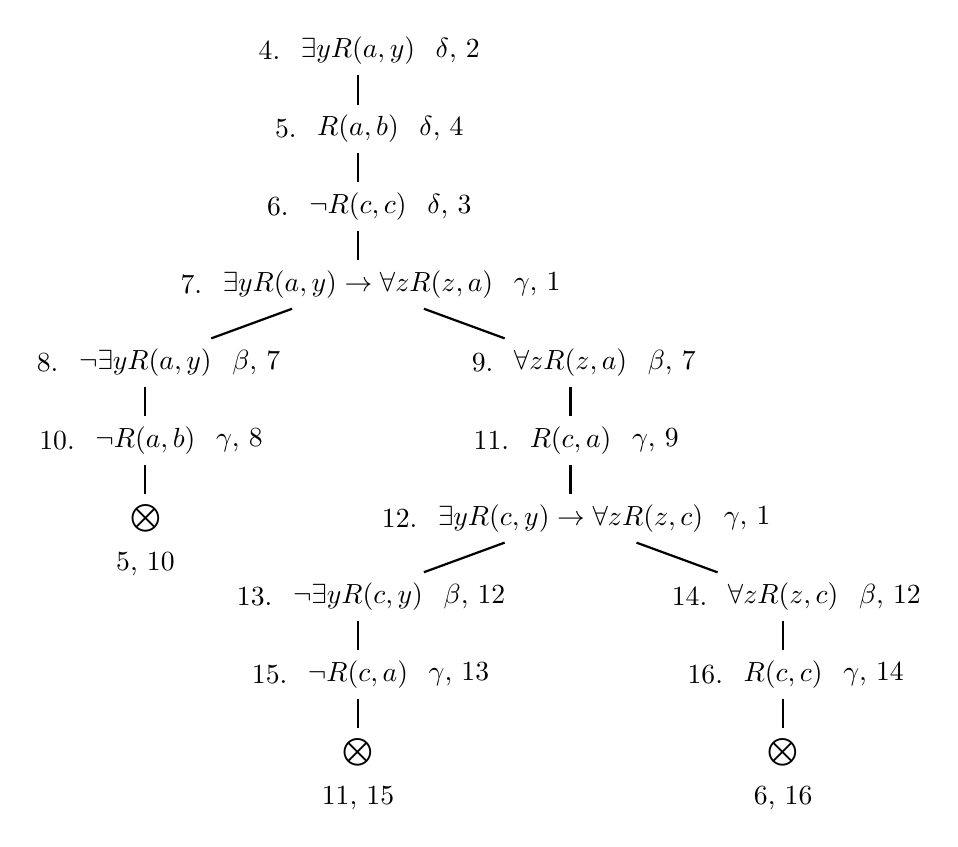
\begin{tikzpicture}[scale=0.9, -, thick, level/.style={sibling distance=6cm,level distance=1.1cm}]
  \node[label=left:{4.},label=right:{$\delta$, 2}] {$\exists y R(a, y)$}
  child {
    node[label=left:{5.},label=right:{$\delta$, 4}] {$R(a, b)$}
    child {
      node[label=left:{6.},label=right:{$\delta$, 3}] {$\neg R(c, c)$}
      child {
        node[label=left:{7.},label=right:{$\gamma$, 1}] {$\exists y R(a, y) \to \forall z R(z, a)$}
        child {
          node[label=left:{8.},label=right:{$\beta$, 7}] {$\neg \exists y R(a, y)$}
          child {
            node[label=left:{10.},label=right:{$\gamma$, 8}] {$\neg R(a, b)$}
            child { node[label=below:{5, 10}] {$\bigotimes$} }
          }
        }
        child {
          node[label=left:{9.},label=right:{$\beta$, 7}] {$\forall z R(z, a)$}
          child {
            node[label=left:{11.},label=right:{$\gamma$, 9}] {$R(c, a)$}
            child {
              node[label=left:{12.},label=right:{$\gamma$, 1}] {$\exists y R(c, y) \to \forall z R(z, c)$}
              child {
                node[label=left:{13.},label=right:{$\beta$, 12}] {$\neg \exists y R(c, y)$}
                child {
                  node[label=left:{15.},label=right:{$\gamma$, 13}] {$\neg R(c, a)$}
                  child { node[label=below:{11, 15}] {$\bigotimes$} }
                }
              }
              child {
                node[label=left:{14.},label=right:{$\beta$, 12}] {$\forall z R(z, c)$}
                child {
                  node[label=left:{16.},label=right:{$\gamma$, 14}] {$R(c, c)$}
                  child { node[label=below:{6, 16}] {$\bigotimes$} }
                }
              }
            }
          }
        }
      }
    }
  };
\end{tikzpicture}
\end{center}
Todas las ramas se cierran: las premisas implican la conclusión. (Como la regla de cierre no exige literales, la rama de 8 podría cerrarse ya con el nodo 4, pues $\neg \exists y R(a, y)$ es la negación de $\exists y R(a, y)$; el paso 10 no es necesario, aunque tampoco es incorrecto).
\end{solucion}

%%% Local Variables:
%%% mode: latex
%%% TeX-master: "ApuntesLogica"
%%% End:
